\documentclass{article}
\usepackage[utf8]{inputenc}
\usepackage[spanish]{babel}
\usepackage{listings}
\usepackage{graphicx}
\graphicspath{ {images/} }
\usepackage{cite}

\begin{document}

\begin{titlepage}
    \begin{center}
        \vspace*{1cm}
            
        \Huge
        \textbf{Desafio 1}
            
        \vspace{0.5cm}
        \LARGE
        Informa2 S.A.S
            
        \vspace{1.5cm}
            
        \textbf{Victor Manuel Jimenez Garcia\\
                Jose Miguel Jaramillo Sanchez\\
                Sebastian Garcia Morales}

        \vfill
            
        \vspace{0.8cm}
            
        \Large
        Despartamento de Ingeniería Electrónica y Telecomunicaciones\\
        Universidad de Antioquia\\
        Medellín\\
        Febrero 17 de 2022
            
    \end{center}
\end{titlepage}

\tableofcontents

\newpage
\section{Objetivos}\label{objetivos}
\begin{itemize}
    \item Aplicar los conocimientos adquiridos a lo largo del curso, demostrando apropiación de los fundamentos básicos del lenguaje de programacion C++.
    \item Desarrollar habilidades de investigación y redacción que permitan la adquisicion de nuevos conocimientos con el fin de solucionar problemas de la vida real.
    \item Demostrar la importancia y utilidad de la programación por hardware, así como el uso de módulos físicos para optimizar el uso de software en un diseño
    \item Diseñar un aplicativo en la plataforma de Arduino integrando programación de C++ para solucionar un desafio  propuesto.
\end{itemize}
\section{Introduccion}\label{intro}
\section{Marco Teorico}\label{marco}

\subsection{Conocimientos previos}

A la hora de enfrentarse a un desafío lo más recomendable es dividirlos en varias etapas para trabajarlo más fácilmente, una primera etapa sería realizar una investigación de conceptos y componentes propuestos en el desafío. En este caso es necesario investigar el concepto de transferir información de forma serial y paralela cómo también identificar características, funcionalidades arquitectura, conexiones, alcances y limitaciones del circuito integrado 75HC595, por otro lado, ¿qué es un Arduino? y ¿cómo unirlo al circuito integrado mencionado anteriormente para lograr solucionar el desafío completo?.\\

Arduino es una plataforma de desarrollo basada en una placa electrónica de hardware libre que incorpora un microcontrolador re-programable y una serie de pines hembra. Estos permiten establecer conexiones entre el microcontrolador y los diferentes sensores y actuadores de una manera muy sencilla (principalmente con cables dupont).\cite{arduinowebsite}\\
Este dispositivo es el que nos permitirá recibir los datos ingresados por el usuario y realizar la conversion a binario, ademas de funcionar tanto transmisor como receptor en el sistema de encriptacion.\\

La comunicacion entre arduinos ser realizará de forma serial, que es el proceso de enviar datos de caracter binario un bit a la vez, esto provee la ventaja de mantener la interfaz transmisor-receptor de forma simple y eficiente.\cite{serialsite}\\
Por lo tanto, para desencriptar, es necesario paralelizar dicha secuencia de bits que luego seran las entradas de un circuito de logica combinacional encargado de comparar los datos de acuerdo a los parametros de desencriptacion.

Paralelizar no es mas que llevar la secuencia de bits que se desplazan como una sola fila, y transformarla en una columna. De esta forma si se tiene una secuencia serial de n bits, al paralelizar, el resultado es una columna de bits de n filas.

\begin{figure}[!ht]
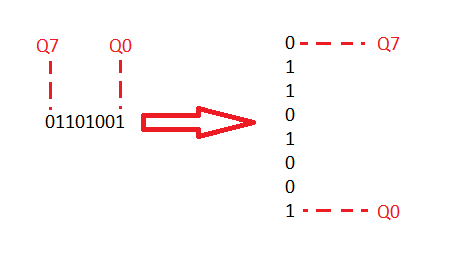
\includegraphics[width=8cm]{paralelizacion.png}
\centering
\caption{Ejemplo de paralelización}
\end{figure}

Esta accion de paralelizar la llevará acabo el circuito integrado 74HC595 tambien conocido como Registro de desplazamiento. Este chip de 16 pines, recibe una secuencia de 8 bits en un solo pin, y los va almacenando en cada una de las salidas para luego ser liberados como 8 señales independientes.\\

Dos definiciones que se deben de tener en cuenta para entender mejor el funcionamiento de todo el sistema son: comunicacion sincrona y comonicacion asincrona.\\

\noindent\textbf{Comunicación sincrónica:} Se da cuando el intercambio de mensajes sucede en tiempo real. Requiere que las dos partes (emisor y receptor) estén presentes en el mismo tiempo y espacio, ya sea físico o virtual. Por ejemplo, las llamadas telefónicas, las reuniones en la oficina o las videoconferencias.\\

\noindent\textbf{Comunicación asincrónica:} Sucede cuando los mensajes se intercambian sin importar el tiempo. Es decir, que no necesitan la atención inmediata del receptor, quien puede responder en el momento que decida o pueda hacerlo. Estamos hablando de medios como el correo electrónico, foros en línea, chats, mensajes de texto y documentos colaborativos.\cite{sincrosite}\\

En este caso, la comunicacion se da de forma sincrona con ayuda de un pulso de reloj.
En electrónica y especialmente en circuitos digitales síncronos, una señal de reloj es una señal usada para coordinar las acciones de dos o más circuitos, esta señal oscila entre estado alto y bajo, tambien conocido como flanco de subida y de bajada, respectivamente, y gráficamente toma la forma de una onda cuadrada.\cite{relojsite}\\

\begin{figure}[!ht]
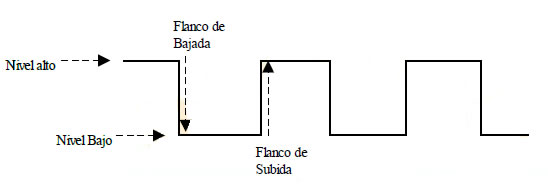
\includegraphics[width=8cm]{flanco1.jpg}
\centering
\caption{Diagrama de tiempo de una señal de reloj}
\end{figure}

A continuacion se muestra la distribucion de pines del circuito integrado 74HC595\\

\begin{figure}[!ht]
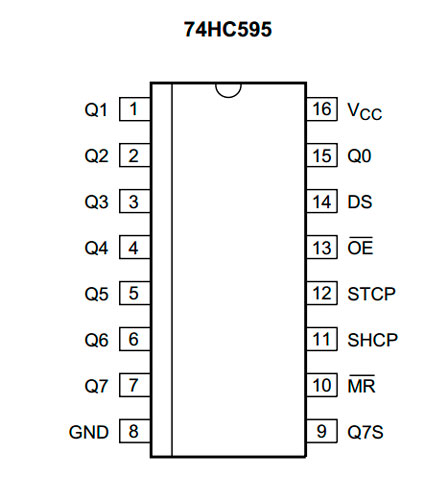
\includegraphics[width=5cm]{74HC595.jpg}
\centering
\caption{Pines IC 74HC595}
\end{figure}

\noindent\textbf{Entradas:}\\
\indent \textbf{GND} (pin 8): conexion a tierra (0 V)\\
\indent \textbf{GND} (pin 10): reinicio del registro (activo bajo)\\
\indent \textbf{SHCP} (pin 11): señal de reloj \\
\indent \textbf{STCP} (pin 12): pulso para liberar los datos \\
\indent \textbf{GND} (pin 13): habilitar salida del registro (activo bajo)\\
\indent \textbf{DS} (pin 14): entrada de datos serial \\
\indent \textbf{VCC} (pin 16): conexion a fuente de voltaje (5 V)\\

\noindent\textbf{Salidas:}\\ 
\indent \textbf{Q0-Q7} (pines 1-7 y 15 ): salida de datos\\
\indent \textbf{Q7S} (pin 9): salida de datos serial\\


El funcionamiento es el siguiente, la informacion serial entra por el \textbf{DS (pin 14)}, el integrado recibe cada bit cuando ocurre un flanco de subida por el \textbf{SHCP (pin 11)} y lo almacena en la salida de mas baja valor \textbf{Q0 (pin 15)}, a medida que van entrando mas bits, los datos que habian almacenados anteriormente se van desplazando desde \textbf{Q0} hasta \textbf{Q7} hasta completar el byte. Una vez hecho esto, se manda un flanco de subida en \textbf{STCP (pin 12)}, que se encargar de liberar los datos almacenados.\\

\noindent De esta forma el primer bit que entra, queda en la salida \textbf{Q7} y el ultimo en la salida \textbf{Q0}.
Para ingresar un nuevo byte se debe borrar la informacion del registro, esto se hace mandando un flanco de bajada al pin \textbf{MR (pin 10)} y luego activando la salida del registro (pin 12).\cite{74hc595datasheet}

\section{Analisis del problema} \label{analisis}

Para afrontar el problema, se opta por dividirlo en distintas etapas o modulos, de forma que se pueda verificar el correcto funcionamiento de cada uno por separado. Una vez hecho esto se juntan todas las etapas para finalmmente construir el modelo final del sistema.\\

Como primera etapa se revisa el funcionamiento del circuito integrado 74HC595 en el simulador Tinkercad con ayuda de leds, botones y suiches. 

Para la alimentacion se usa una fuente de voltaje de 5 V, se realizan las respectivas conexiones de forma que cada led represente una salida del integrado y por facilidad se realiza el montaje solo para 4 bits. Las funciones de reloj, datos, y liberacion de datos se realizan con suiches y botones.\\

Para ingresar un dato se usa el boton reloj, que permitirá la entrada de un 1 o un 0, de acuerdo a la posicion que tenga el suiche deslizante (la izquierda representa 1 y la derecha 0). Luego de tener 4 datos ingresados se presiona el boton reloj de registro, mostrando los datos ingresados en los leds.

Una vez montado el circuito, se evidencia que, aunque su comportamiento es el esperado, no se permitía ingresar mas información nueva ni borrar la existente, esto se debía a que no se había agregado un boton de reset en el pin 10 del integrado.

\begin{figure}[!ht]
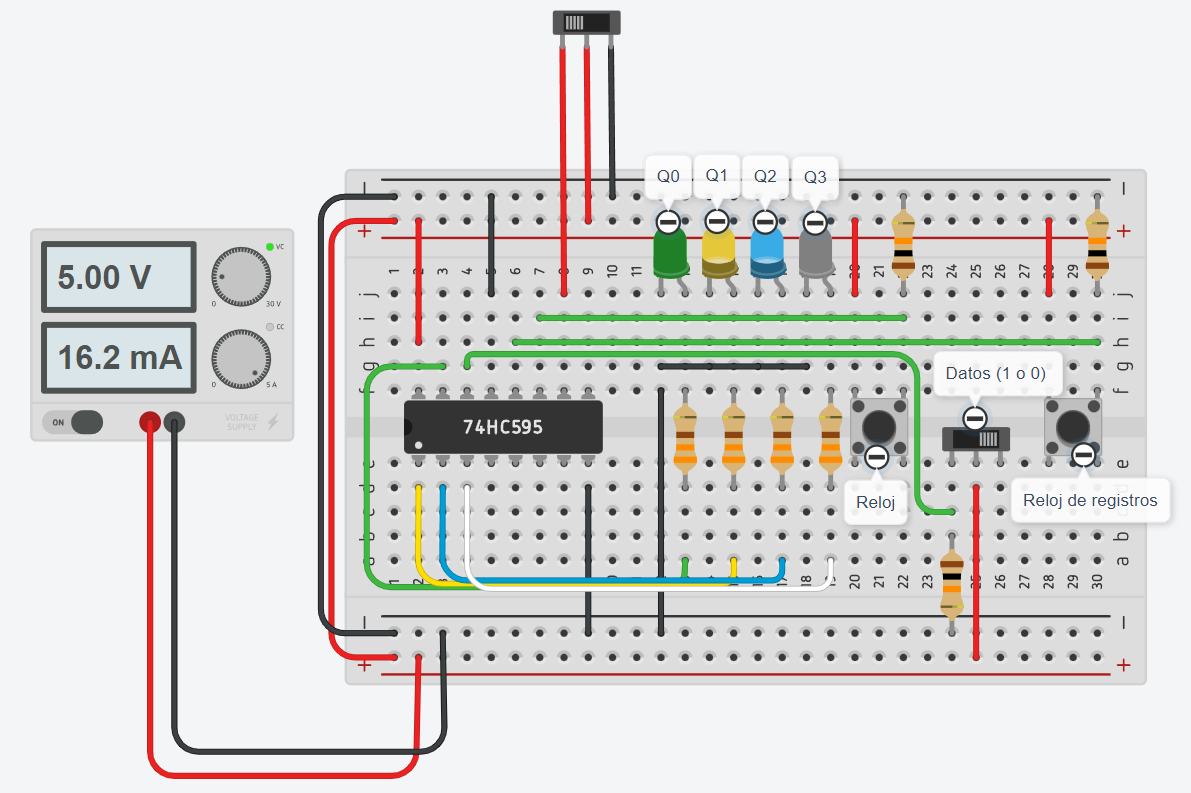
\includegraphics[width=10cm]{montaje0.PNG}
\centering
\caption{Primer montaje con el 74HC595}
\end{figure}

Despues de haber garantizado el funcionamiento con botones y suiches, se procede a reemplazarlos por las salidas digitales del Arduino, en este caso el reset, el reloj de registro, la entrada de datos y el reloj estan conectados a los pines 4, 5, 6 y 7 respectivamente. Tambien se usan leds adicionales para llevar control de los pulsos que salen del Arduino.

\begin{figure}[!ht]
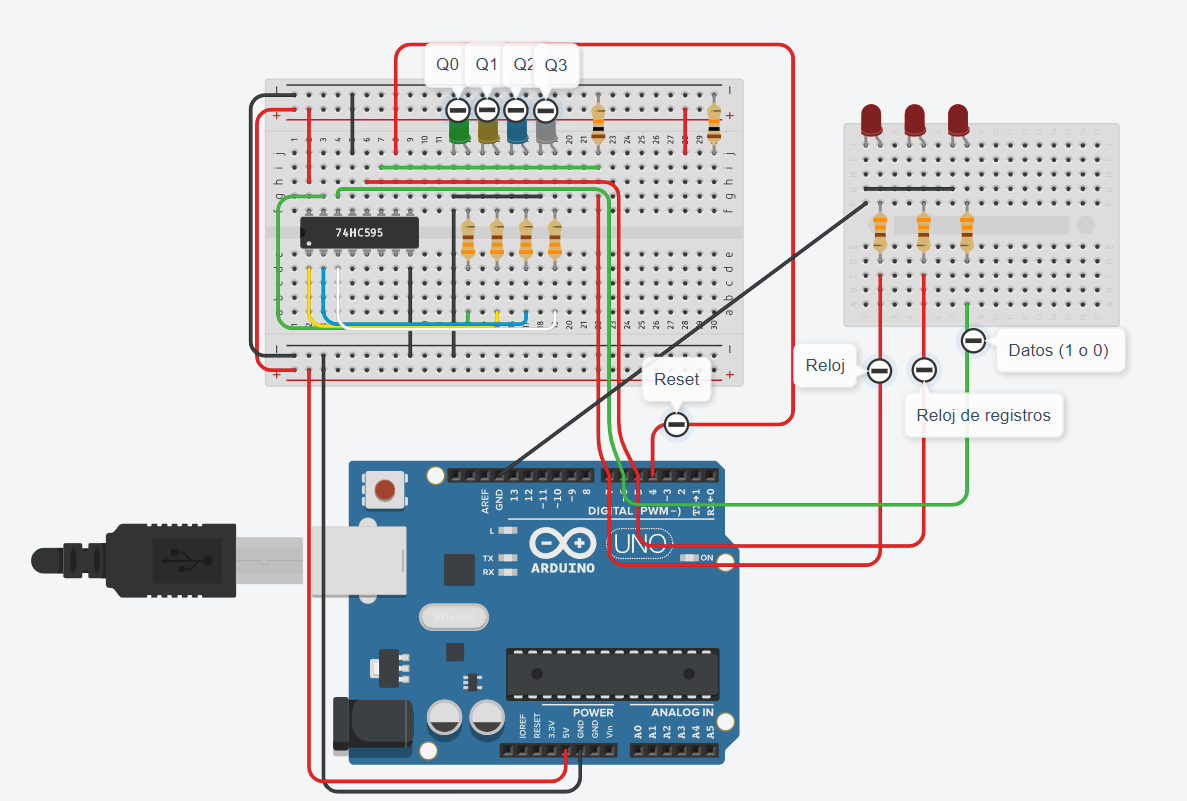
\includegraphics[width=10cm]{montaje1.PNG}
\centering
\caption{Montaje con 74HC595 y Arduino}
\end{figure}



\section{Conclusiones} \label{conclusiones}


\bibliographystyle{IEEEtran}
\bibliography{references}

\end{document}
